\subsection{Environmental Permit Application Process}
\label{subsec:coselog-wabo-process}

In \textit{Environmental Permit Application Process} dataset \cite{coselog-data}, there are total of 1214 cases and 2142 events with a variable distribution between event logs of municipalities and municipalities are used as organizational logs.

\begin{itemize}
  \item In \textit{Process Model Mining} stage, with 10\% of noise threshold, high fitness values are achieved; however, some of the process models like Municipality \#5 and \#4 resulted with low appropriateness values. 
  \item In \textit{Performance Indicator Analysis} stage, after calculating the performance indicators, municipalities are clustered based on these values and three clusters are created, Municipality \#1 is located in the first cluster; Municipality \#2 and \#4 are located in the second cluster; and Municipality \#3 and \#5 are grouped in to the last cluster.
  \item In \textit{Mismatch Pattern Analysis} stage, it can be stated that as the similarity between process models of municipalities increases, number of mismatch patterns decreases on most of the cases. When further analyzed, it can be seen that Municipalities \#4 and \#5, which have significantly more complex process model compared to others, fails in spotting mismatch patterns according to \textit{graph-edit similarity}.
  \item In \textit{Recommendation Generation} stage, an organization and performance difference threshold is selected as analysis input likewise the previous dataset. For different threshold values, number of performance indicators that are performing better for the selected organization and spotted mismatch patterns are plotted in Figure~\ref{fig:coselog-wabo-recommendation-generation-analysis} for the thresholds of 25 \%, 50 \% and 75 \% since these are the breaking points for performance indicator changes. As plotted in Figure~\ref{fig:coselog-wabo-recommendation-generation-analysis-k3}, in addition to Municipality \#1, now Municipality \#3 and \#5 have the learning potential from other clusters. However, Municipality \#2 and \#4 performs better in all performance indicators which yielded no mismatch pattern analysis data for them. Increasing cluster sizes in this analysis shows that organizations can learn more from each other but it has the potential danger of overfitting to other organizations process model. 
	\begin{figure}
		\centering
		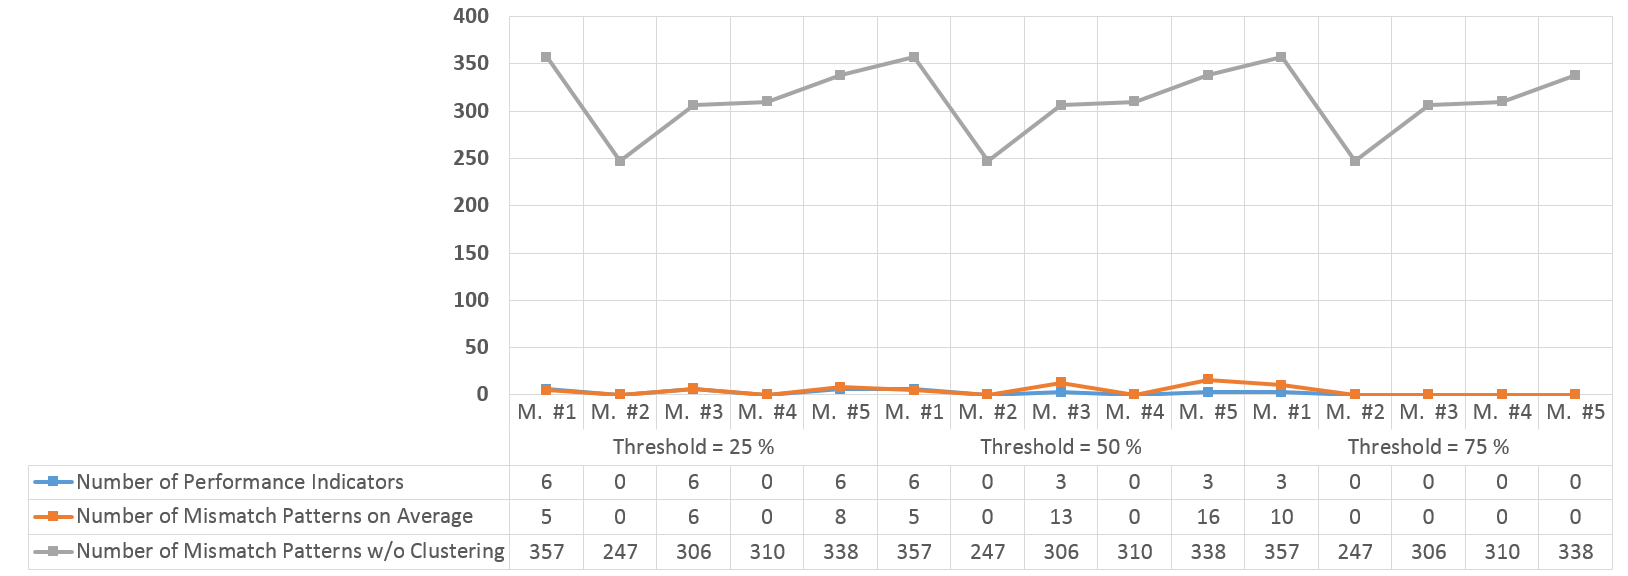
\includegraphics[width=\textwidth]{5_results_discussions/coselog-wabo/recommendation-generation-analysis-k3}
		\caption{Recommendation Generation analysis for Environmental Permit Application Process dataset (3 Clusters)}
	  \label{fig:coselog-wabo-recommendation-generation-analysis-k3}
	\end{figure}
\end{itemize}
